\documentclass[11pt, oneside]{article}   	% use "amsart" instead of "article" for AMSLaTeX format
\usepackage{geometry}                		% See geometry.pdf to learn the layout options. There are lots.
\geometry{letterpaper}                   		% ... or a4paper or a5paper or ... 
%\geometry{landscape}                		% Activate for for rotated page geometry
%\usepackage[parfill]{parskip}    		% Activate to begin paragraphs with an empty line rather than an indent
\usepackage{graphicx}				% Use pdf, png, jpg, or eps� with pdflatex; use eps in DVI mode
								% TeX will automatically convert eps --> pdf in pdflatex		
\usepackage{amssymb}

\title{A Microfluidic Device for Measuring Aerotaxis}
\author{Kiarash Adl, Brian Djaja, Katarina Struckmann and Logan Williams}
%\date{}							% Activate to display a given date or no date

\begin{document}
\maketitle
%\section{}
%\subsection{}
\section{Abstract}

Bacteria rely heavily on sensing environmental gradients to survive and reproduce. While significant effort has been made to understand responses to chemical gradients, or chemotactic responses, less literature exists characterizing responses to gas gradients, or aerotactic responses. This study employed a three-channel microfluidic device fabricated from PDMS to characterize aerotactic bacterial motion. In the presence of a gradient of nitrogen and oxygen, movement of the organism \textit{B. subtilis} tended toward oxygen and away from nitrogen, demonstrating an aerotactic response.

\section{Introduction}

The movement of bacteria in response to a gas gradient, aerotaxis, is a field that has emerged within the past 10 years. As such, it has not been studied to the extent of the similar process chemotaxis. Chemotaxis is the movement of bacteria in response to a chemical gradient, where the chemical can be anything from food to toxic molecules. Models for chemotaxis in bacteria have been characterized, both for populations and single bacterial cells.2,3

Aerotaxis was studied in a microfluidic device using a custom optical microscope. The microfluidic device allowed for development of a gas gradient along its length; the bacteria�s response to the gradient was visualized with the microscope. This setup can be utilized for studying different bacteria species and potentially other cell types. 

Aerotaxis has a broad range of applications; the signaling proteins utilized in for aerotactic responses in bacteria can be potentially engineered for turning on gene expression in the presence of a certain oxygen concentration, or lack thereof. Since aerotaxis occurs on the order of minutes, a response can be expressed fairly quickly. Additionally, modeling aerotaxis is key to understanding how applications such as the aforementioned can be utilized.

\section{Experimental apparatus}
\subsection{The microscope} % Logan or Kiarash?
\subsection{The microfluidic device} % Logan or Kiarash?
\subsection{Gas flow} % Kat?
\subsection{Bacteria culturing} % Brian?
\section{Results} % all of us

\begin{figure}[h!] 
  \centering
    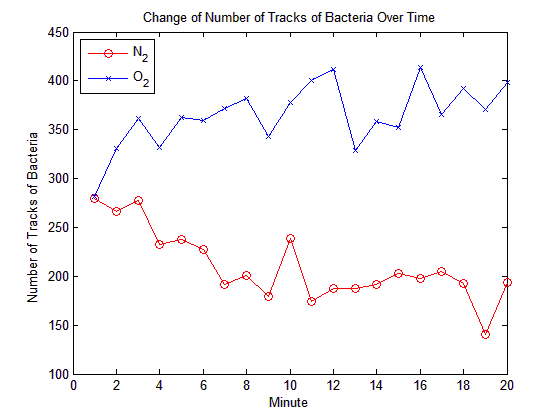
\includegraphics[width=\textwidth]{plots/number_Tracks.png}
      \caption[Number of trackable bacteria]{The number of trackable bacteria adjacent on the nitrogen side of the channel as compared to the number on the oxygen side. \\
      
      To obtain this data, an experiment was conducted where \emph{B. subtilis} was injected into the central channel, and oxygen and nitroge
      
      This plot was produced by finding bright centroids in captured microscope frames, and tracking the motion of the centroids. The number of ``tracks'' produced corresponds to the number of trackable bacteria.}
\end{figure}

\begin{figure}[h!] 
  \centering
    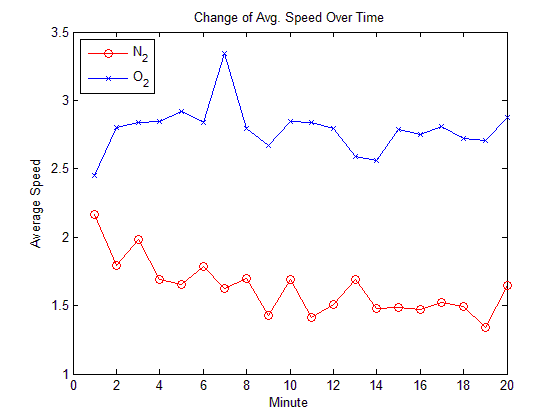
\includegraphics[width=\textwidth]{plots/average_speed.png}
      \caption[Number of trackable bacteria]{The speed of trackable bacteria adjacent on the nitrogen side of the channel as compared to the number on the oxygen side. \\
      
      This plot was produced by finding bright centroids in captured microscope frames, and tracking the motion of the centroids. The speed of each track corresponds to the average displacement of the centroid from frame to frame}
\end{figure}

\begin{figure}[h!] 
  \centering
    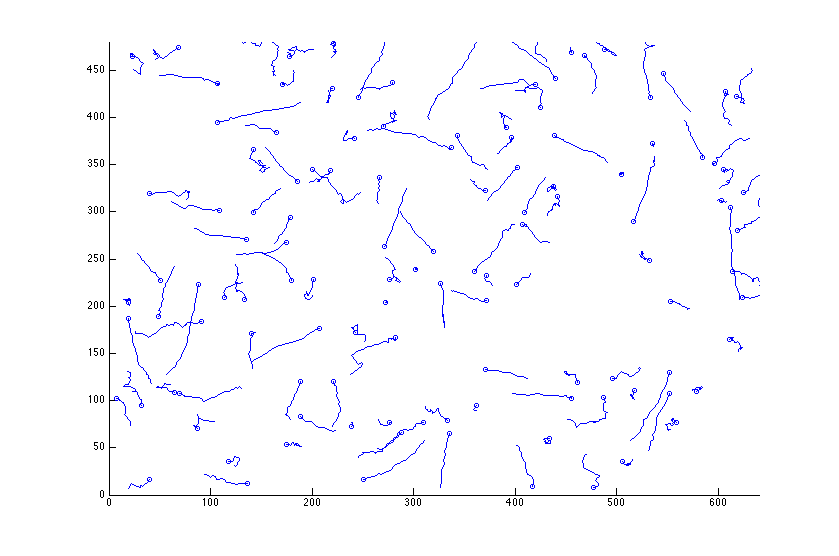
\includegraphics[width=0.5\textwidth]{plots/tracks_1.png}
    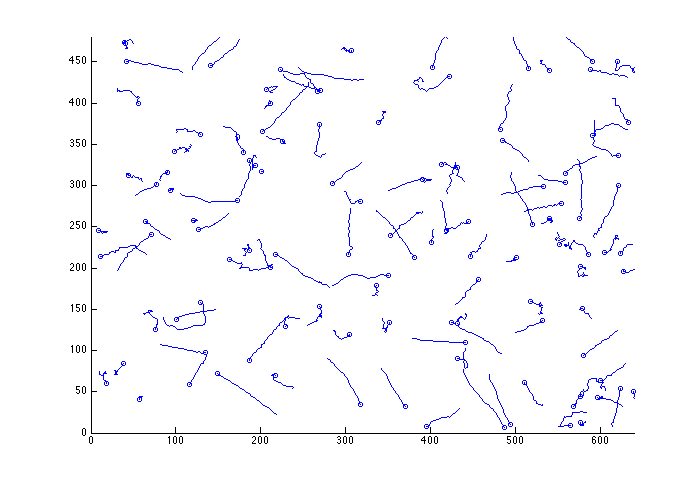
\includegraphics[width=0.5\textwidth]{plots/tracks_2.png}
    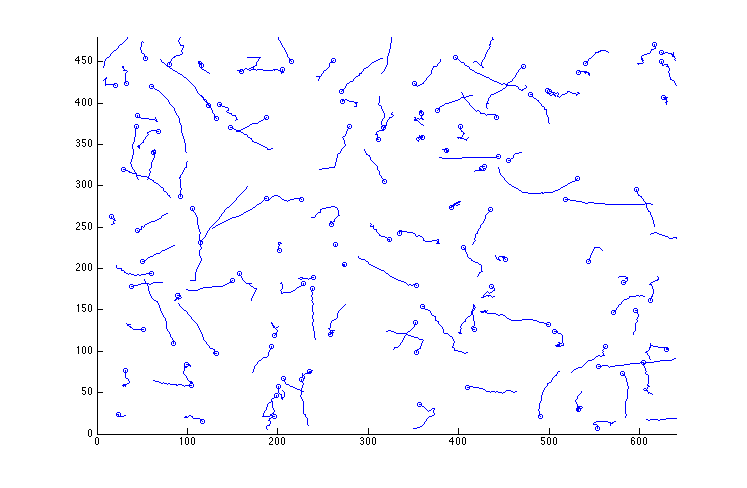
\includegraphics[width=0.5\textwidth]{plots/tracks_3.png}
      \caption[Representative traces]{Representative traces of bacteria motion. \\
      
      These plots were produced by finding bright centroids in captured microscope frames, and then finding centroids in sequential frames that are likely to belong to the same bacteria. These are plotted prior to gas flow switch, just after gas flow switch, and several minutes after gas flow switch, though no difference is apparent visually.}
\end{figure}

\begin{figure}[h!] 
  \centering
    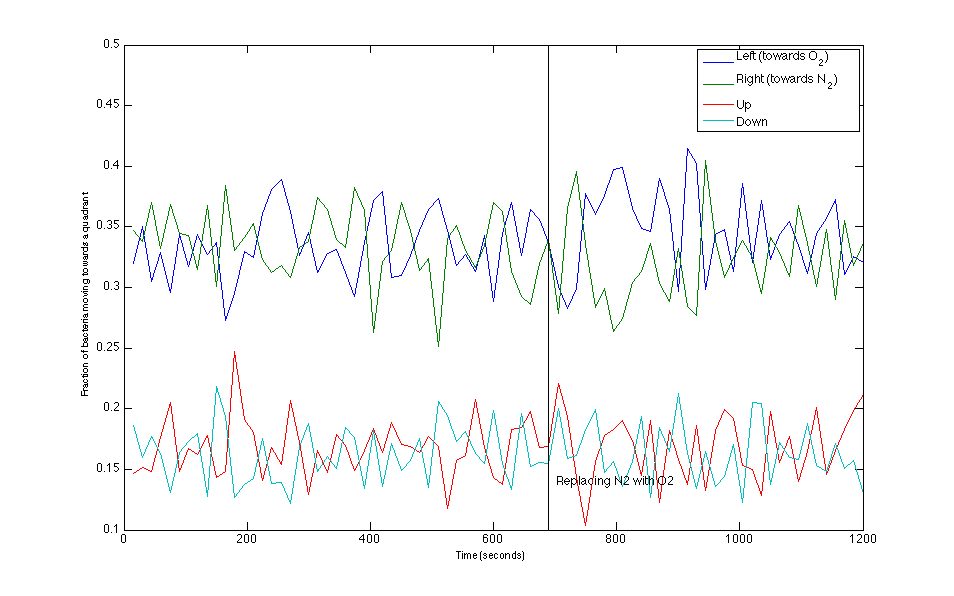
\includegraphics[width=\textwidth]{plots/direction.png}
      \caption[Bacterial motion]{Motion of motile bacteria divided into four quadrants, left (towards oxygen), right (towards nitrogen, up, and down.) This shows data from one representative experiment. \\
      
      This graph was produced by calculating the distance traveled and direction of travel for every bacteria ``track'' in each sequence of 30 frames. Bacteria that moved a significant amount were considered ``motile,'' all other bacteria were discarded. The bacteria were divided by dividing their motion into the four previously mentioned quadrants.}
\end{figure}

\begin{figure}[h!] 
  \centering
    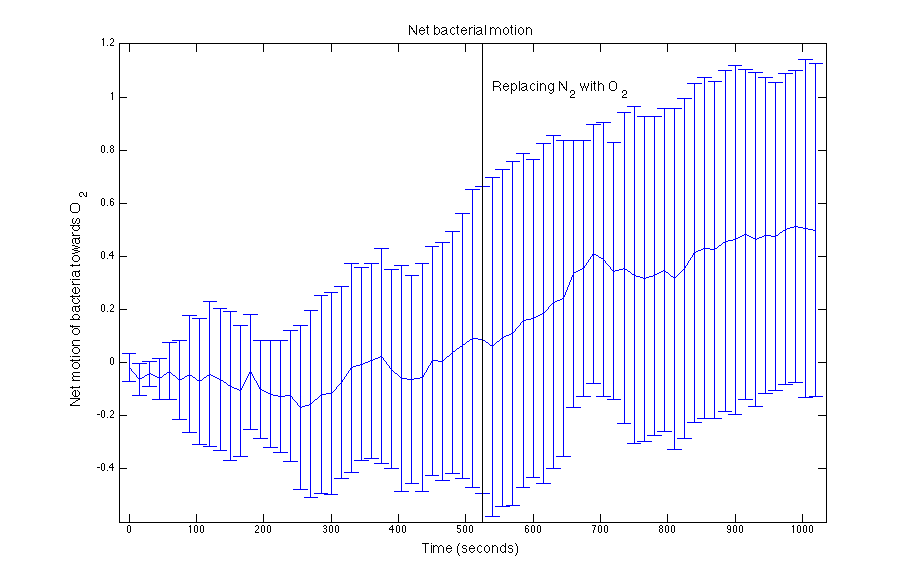
\includegraphics[width=\textwidth]{plots/cum_motion.png}
	\caption[Cumulative motion]{The cumulative percentage of net bacterial movement towards the oxygen side of the channel, averaged over 5 experimental trials. The x-axis is scaled relative to the number of visible bacteria in a single frame. \\
      
      This plot was produced by taking the cumulative sum of the difference between the ``left'' and ``right'' quadrants in the preceding figure. This sum is averaged over five trials. Error bars represent the standard deviation of that cumulative sum over the five trials (they grow with time because error is also being integrated in the cumulative sum). The size of the error bars is caused by a small $n$ (5), and integrated error. \\
      
      Note that there appears to be some drift prior to the gas line switch. This is likely due to random motion of the bacteria, and the large uncertainty in the data.}
      
\end{figure}


\section{Discussion} % all of us


\end{document}  